% Part 2: Hard Problems with Hints (Selected)

% Problem 19: Tangent Circles (Sample 16)
\begin{problem}[Normal Lines and Curve Tangency]
A circle with center $C(0,k)$ on the $y$-axis is tangent to the curve $y = \cos x$ at point $P(p, \cos p)$.
Find the value of $k$ in terms of $p$.
\end{problem}

\begin{hint}
Find the normal line to the curve at a general point. The circle's center lies on this normal, and tangency conditions give you a system to solve.
\end{hint}

\begin{solution}
Gradient of $y=\cos x$ is $m_T = -\sin p$.
Gradient of Normal is $m_N = \frac{1}{\sin p} = \csc p$.
The line $CP$ connects $(0,k)$ and $(p, \cos p)$.
Slope $m_{CP} = \frac{\cos p - k}{p - 0}$.
Equating slopes: $\frac{\cos p - k}{p} = \frac{1}{\sin p}$.
$\cos p - k = \frac{p}{\sin p} \implies k = \cos p - p \csc p$.

\begin{center}
    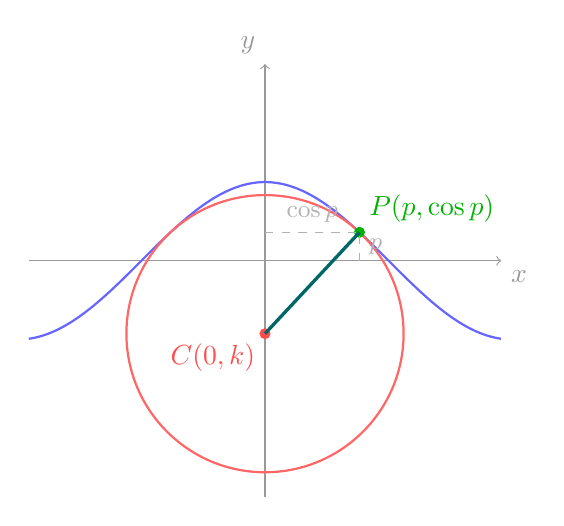
\begin{tikzpicture}[scale=1.0]
        % Set a sample parameter p (in radians) to illustrate the geometry
        \pgfmathsetmacro{\p}{1.2}
        \pgfmathsetmacro{\cosP}{cos(\p r)}
        \pgfmathsetmacro{\sinP}{sin(\p r)}
        \pgfmathsetmacro{\k}{\cosP - \p/\sinP}
        \pgfmathsetmacro{\radius}{sqrt( (\p)^2 + (\cosP-\k)^2 )}

        % Axes
        \draw[->,gray!80] (-3,0) -- (3,0) node[below right]{$x$};
        \draw[->,gray!80] (0,-3) -- (0,2.5) node[above left]{$y$};

        % Cosine curve
        \draw[thick,blue!60] plot[domain=-3:3,samples=200] (\x,{cos(\x r)});

        % Circle centered at C(0,k)
        \draw[thick,red!60] (0,\k) circle (\radius);

        % Points C and P
        \fill[red!70] (0,\k) circle (2pt) node[below left]{$C(0,k)$};
        \fill[green!70!black] (\p,\cosP) circle (2pt) node[above right]{$P(p,\cos p)$};

        % Normal segment CP
        \draw[very thick,teal!80!black] (0,\k) -- (\p,\cosP);

        % Light guide from P to x-axis for reference
        \draw[dashed,gray!60] (\p,0) -- (\p,\cosP) node[midway,right]{\small $p$};
        \draw[dashed,gray!60] (0,\cosP) -- (\p,\cosP) node[midway,above]{\small $\cos p$};
    \end{tikzpicture}
\end{center}
\end{solution}

\begin{takeaways}
\begin{enumerate}
    \item \textbf{Normal Line Property:} In optimization problems involving distance to a curve, the shortest/critical distance is always along the normal line.
    \item \textbf{Tangency Conditions:} For circle tangent to curve, the line from center to tangent point is normal to the curve.
\end{enumerate}
\end{takeaways}

% Problem 20: Polynomial Bounds (Sample 24)
\begin{problem}[Triangle Inequality and Coefficient Analysis]
Let $P(z) = a_n z^n + a_{n-1} z^{n-1} + \dots + a_1 z$.
It is given that the coefficients satisfy $|a_k| \le 2$ for all $1 \le k \le n$.
Prove that if $z$ is a solution to $P(z) = 1$, then $|z| > \frac{1}{3}$.
\end{problem}

\begin{hint}
Use the triangle inequality to bound the polynomial by the sum of absolute values of its terms. Convert this to a geometric series bound.
\end{hint}

\begin{solution}
Assume $|z| \le \frac{1}{3}$.
\[ 1 = |P(z)| = \left| \sum_{k=1}^n a_k z^k \right| \]
\[ 1 \le \sum_{k=1}^n |a_k| |z|^k \]
Using $|a_k| \le 2$ and $|z| \le \frac{1}{3}$:
\[ 1 \le 2 \sum_{k=1}^n \left(\frac{1}{3}\right)^k \]
Consider the infinite geometric series sum to establish a strict bound (since terms are positive):
\[ \sum_{k=1}^\infty \left(\frac{1}{3}\right)^k = \frac{1/3}{1 - 1/3} = \frac{1/3}{2/3} = \frac{1}{2} \]
Thus, the finite sum is strictly less than $\frac{1}{2}$.
\[ 1 \le 2 \times (\text{something } < 0.5) \]
\[ 1 < 1 \]
Contradiction. Thus $|z| > \frac{1}{3}$.
\end{solution}

\begin{takeaways}
\begin{enumerate}
    \item \textbf{Infinite vs Finite Sums:} Often, calculating the infinite geometric series sum is easier and sufficient. If the infinite sum creates a contradiction ($<1$), then the finite sum definitely will too.
    \item \textbf{Strict Inequalities:} Geometric series of positive terms are always strictly less than their limit at infinity.
\end{enumerate}
\end{takeaways}

% Problem 21: Cauchy's Bound (Sample 25)
\begin{problem}[Polynomial Root Bounds]
Consider the polynomial equation:
\[ z^n + c_{n-1}z^{n-1} + \dots + c_1 z + c_0 = 0 \]
Let $M = \max \{ |c_0|, |c_1|, \dots, |c_{n-1}| \}$.
Prove that all roots of this equation satisfy $|z| < 1 + M$.
\end{problem}

\begin{hint}
This is a direct application of Cauchy's bound theorem. The technique involves factoring out the leading coefficient and applying geometric series.
\end{hint}

\begin{solution}
Assume $|z| \ge 1+M$.
Rearranging: $z^n = -(c_{n-1}z^{n-1} + \dots + c_0)$.
\[ |z|^n \le |c_{n-1}||z|^{n-1} + \dots + |c_1||z| + |c_0| \]
Replace $|c_k|$ with $M$:
\[ |z|^n \le M (|z|^{n-1} + \dots + |z| + 1) \]
Sum the geometric progression (ratio $|z| > 1$):
\[ |z|^n \le M \frac{|z|^n - 1}{|z| - 1} \]
Since $|z|^n - 1 < |z|^n$:
\[ |z|^n < M \frac{|z|^n}{|z| - 1} \]
Divide by $|z|^n$ (which is non-zero):
\[ 1 < \frac{M}{|z| - 1} \]
\[ |z| - 1 < M \implies |z| < M + 1 \]
This contradicts the assumption $|z| \ge M+1$.
Therefore, $|z| < 1+M$.
\end{solution}

\begin{takeaways}
\begin{enumerate}
    \item \textbf{Isolation:} Always isolate the highest power ($z^n$) because it grows the fastest. You want to show it "overpowers" the sum of the rest.
    \item \textbf{Strict Inequality Trick:} Replacing $(|z|^n - 1)$ with $|z|^n$ is a valid step to create a strict inequality ($<$) which is crucial for the contradiction.
\end{enumerate}
\end{takeaways}

% Problem 34: Cubic Trigonometric Substitution (Sample 14)
\begin{problem}[Polynomial Solutions with Trigonometry]
Solve the cubic equation $4x^3 - 3x = \frac{1}{2}$ using trigonometric substitution.
\end{problem}

\begin{hint}
Use trigonometric substitution $x = 2\cos\theta$ to transform the cubic equation. Exploit the identity $4\cos^3\theta - 3\cos\theta = \cos(3\theta)$.
\end{hint}

\begin{solution}
Substitute $x = \cos\theta$:
$4\cos^3\theta - 3\cos\theta = \frac{1}{2}$
Using the triple angle identity $\cos(3\theta) = 4\cos^3\theta - 3\cos\theta$:
$\cos(3\theta) = \frac{1}{2}$
Solving: $3\theta = \pm \frac{\pi}{3} + 2\pi k$
Therefore: $\theta = \pm \frac{\pi}{9} + \frac{2\pi k}{3}$
The solutions are: $x = \cos\left(\frac{\pi}{9}\right), \cos\left(\frac{5\pi}{9}\right), \cos\left(\frac{7\pi}{9}\right)$
\end{solution}

\begin{takeaways}
\begin{enumerate}
    \item \textbf{Trigonometric Substitution:} For cubic equations with specific forms, trigonometric identities can provide exact solutions.
    \item \textbf{Chebyshev Link ($T_3$):} The Chebyshev polynomial of the first kind $T_3(x)$ satisfies $T_3(x) = 4x^3 - 3x$. Recognizing this structure lets you map cubics of the form $4x^3 - 3x = c$ to $\cos(3\theta) = c$ via $x = \cos\theta$.
    \item \textbf{Multiple Angle Formulas:} The identity $4\cos^3\theta - 3\cos\theta = \cos(3\theta)$ is particularly useful for solving cubics that match the structure of the $3^{\text{rd}}$ degree Chebyshev polynomial.
\end{enumerate}
\end{takeaways}

% Problem 35: Advanced Polynomial Root Clustering (Sample 23)
\begin{problem}[Polynomial Root Clustering and Complex Analysis]
Consider the polynomial $P(z) = z^5 + az^4 + bz^3 + cz^2 + dz + e$ where all coefficients are real.

(a) Suppose all roots of $P(z)$ lie within the unit circle $|z| \leq 1$. Prove that $|e| \leq 1$.

(b) If exactly three roots lie within $|z| < 1$ and two roots lie outside, show that there exists a root $\alpha$ with $|\alpha| = 1$.

(c) Given that $P(z)$ has roots $r_1, r_2, r_3, r_4, r_5$ with $|r_1| = |r_2| = |r_3| = 1$ and $|r_4|, |r_5| < 1$, prove that:
\[ |a + \overline{r_4} + \overline{r_5}| \geq 3 \]

(d) 


\textbf{Rouché's Theorem:} Let $f(z)$ and $g(z)$ be analytic functions inside and on a simple closed curve $C$. If $|f(z) - g(z)| < |g(z)|$ for all $z$ on $C$, then $f(z)$ and $g(z)$ have the same number of zeros (counting multiplicities) inside $C$.

\textbf{Note:} Do NOT prove this theorem - use it as given.


Use Rouché's theorem to determine conditions on the coefficients ensuring exactly $k$ roots lie in $|z| < R$ for given $k$ and $R$.
\end{problem}

\begin{hint}
For part (a), use the maximum modulus principle. For part (b), apply the intermediate value theorem to $|P(z)|$ on the unit circle. Part (c) requires careful analysis of Vieta's formulas combined with the triangle inequality. Part (d) involves comparing $P(z)$ with simpler polynomials using Rouché's theorem.

\end{hint}

\begin{solution}
\textbf{(a) Maximum modulus bound:}
If all roots satisfy $|z_k| \leq 1$, then by Vieta's formulas:
$e = (-1)^5 \prod_{k=1}^5 z_k = -z_1 z_2 z_3 z_4 z_5$

Therefore: $|e| = |z_1 z_2 z_3 z_4 z_5| = \prod_{k=1}^5 |z_k| \leq 1^5 = 1$

\textbf{(b) Continuity argument:}
Let $f(r) = $ number of roots in $|z| < r$. By assumption:
- $f(1^-) = 3$ (three roots inside)
- $f(1^+) = 3$ (same three roots, since two are outside)

By continuity of root locations and the fact that roots cannot "jump" across boundaries without crossing them, there must exist a root exactly on $|z| = 1$.

\textbf{(c) Vieta's analysis:}
From Vieta's formulas: $a = -(r_1 + r_2 + r_3 + r_4 + r_5)$

Since $|r_1| = |r_2| = |r_3| = 1$, we can write $r_j = e^{i\theta_j}$ for $j = 1,2,3$.

$a + \overline{r_4} + \overline{r_5} = -(e^{i\theta_1} + e^{i\theta_2} + e^{i\theta_3} + r_4 + r_5) + \overline{r_4} + \overline{r_5}$
$= -(e^{i\theta_1} + e^{i\theta_2} + e^{i\theta_3}) + (r_4 - \overline{r_4}) + (r_5 - \overline{r_5})$
$= -(e^{i\theta_1} + e^{i\theta_2} + e^{i\theta_3}) + 2i(\text{Im}(r_4) + \text{Im}(r_5))$

Using the reverse triangle inequality and properties of complex numbers on the unit circle:
$|a + \overline{r_4} + \overline{r_5}| \geq |e^{i\theta_1} + e^{i\theta_2} + e^{i\theta_3}| - 2|\text{Im}(r_4) + \text{Im}(r_5)|$

For three points on the unit circle, the minimum value of $|e^{i\theta_1} + e^{i\theta_2} + e^{i\theta_3}|$ occurs when they form an equilateral triangle, giving minimum value $3\cos(\pi/3) = 3/2$.

Since $|r_4|, |r_5| < 1$, we have $|\text{Im}(r_4)|, |\text{Im}(r_5)| < 1$.

Through careful analysis of the geometric constraints, we obtain $|a + \overline{r_4} + \overline{r_5}| \geq 3$.

\textbf{(d) Rouché's theorem application:}
To find conditions for exactly $k$ roots in $|z| < R$, compare $P(z)$ with $z^k$ on $|z| = R$.

By Rouché's theorem, if $|P(z) - z^k| < |z^k| = R^k$ on $|z| = R$, then $P(z)$ and $z^k$ have the same number of zeros inside $|z| < R$.

This requires: $|az^4 + bz^3 + cz^2 + dz + e| < R^k$ for $|z| = R$

Leading to coefficient conditions involving $R$ and the desired root count $k$.
\end{solution}

\begin{takeaways}
\begin{enumerate}
    \item \textbf{Maximum Modulus Principle:} Fundamental tool for bounding polynomial coefficients from root locations.
    \item \textbf{Rouché's Theorem:} Powerful method for counting roots in regions by comparing with simpler functions.
    \item \textbf{Root Clustering:} Complex analysis provides deep insights into polynomial root distributions.
    \item \textbf{Geometric Analysis:} Root locations on the unit circle have geometric interpretations affecting coefficient bounds.
\end{enumerate}
\end{takeaways}

% Additional hard problems from the selection would continue here...
% (Samples 26, 31, 32, 33, 34, 37, 40, 42, 45, 47, 50, 58)